\documentclass[10pt]{beamer}
\setbeamertemplate{navigation symbols}{}

\usepackage{physics}
\usefonttheme{serif}
\usetheme{Madrid}
\usecolortheme{whale}
\graphicspath{{results/}}
\usepackage{caption}
\captionsetup{font=footnotesize}
%\setbeamercolor{background canvas}{bg=black!30}

\title{Machine Learning in Particle Physics}
\subtitle{Correzione alle Energie di Raggi Cosmici}
\author[R. Di Loreto]{Roberto Di Loreto}
\institute[UNIVAQ]{Università degli Studi dell'Aquila}
\date{\today}

\begin{document}

\begin{frame}
	\titlepage
\end{frame}

\begin{frame}{Introduzione}

Lo scopo di questo progetto è quello di mostrare come i metodi di Machine Learning (ML) possano aiutare a comprendere meglio la fisica che si cela dietro i \emph{raggi cosmici}.
\bigskip

L'idea è analizzare i dati del Pierre Auger Observatory per studiare la ricostruzione dell'energia dei raggi cosmici. Queste particelle trasportano energie milioni di volte superiori a quelle raggiungibili al Large Hadron Collider, offrendo una finestra unica su fenomeni astrofisici estremi. \bigskip

Il metodo di ricostruzione noto come Constant Intensity Cut (CIC) ha alla base delle assunzioni fisiche particolari e non sempre vere.\\ Grazie al ML si può correggere questa ricostruzione e vedere dove il modello tipico fallisce. 

\end{frame}

\begin{frame}{Raggi cosmici}

I raggi cosmici sono particelle cariche, principalmente protoni o nuclei atomici, che bombardano costantemente la Terra provenendo dallo spazio.\bigskip

La loro origine è un mistero che si infittisce alle energie più estreme. Quando una di queste particelle, con energie superiori a $10^{18}$ eV, colpisce l'atmosfera terrestre, genera una cascata di miliardi di particelle secondarie nota come "sciame esteso dell'atmosfera".\bigskip

La loro estrema rarità rende necessario un rivelatore di dimensioni senza precedenti. È qui che entra in gioco l'Osservatorio Pierre Auger, situato nella Pampa Amarilla in Argentina.\\
Con una superficie di $3000\ km^2$ , è il più grande rivelatore di raggi cosmici al mondo.

\end{frame}

\begin{frame}{Pierre Auger Open Data}

La forza dell'osservatorio Auger risiede nel design "ibrido": combina un rivelatore di superficie (Surface Detector, SD), composto da 1660 serbatoi d'acqua distribuiti su una griglia, con un rivelatore a fluorescenza (Fluorescence Detector, FD), che osserva la luce ultravioletta emessa durante lo sviluppo dello sciame in atmosfera. 
\bigskip

I dati raccolti da questi detector sono accessibili pubblicamente attraverso il loro portale web. Sono messi a disposizione sia i "raw data" di ogni singolo evento, sia un file di sintesi (summary.csv), contenente eventi sottoposti a selezioni ferree (circa il 10\% di quelli raccolti) e con le sole variabili principali.
\bigskip

Il lavoro è stato svolto su quest'ultimo, in particolare sulla parte contenente i dati raccolti dalla griglia di rivelatori distanti $750\ m$ l'uno dall'altro (SD750). La densità di stazioni consente una ricostruzione più accurata, riducendo le incertezze dovute a fluttuazioni stocastiche.
\end{frame}

\begin{frame}{Struttura dei dati}

Il dataframe contiene 54482 eventi (righe); per ognuno si registrano 72 variabili (colonne), divise in quelle registrate da SD e FD attraverso la dicitura \texttt{sd\_[nome variabile]}, \texttt{fd\_[nome variabile]}.
\bigskip

Non tutti gli eventi presentano misure dei due tipi di rivelatori. Quelli che hanno una riga completa sono noti come \emph{Golden Hybrids}.  Gli eventi di questo tipo sono di grande valore poiché hanno superato criteri di selezione di ben due classi di rivelatori. In generale possono essere gli eventi di base per una corretta calibrazione dei modelli ML.
\bigskip

Il dataframe è stato ridotto dunque a 31 variabili, le quali sono state suddivise in info (7), variabili del SD (17) ed errori associati alle misure (7). \\

\end{frame}

\begin{frame}{Metodo CIC}
Tra le variabili del dataframe, la più importante per ricostruire l'energia dei raggi cosmici è \texttt{sd\_s450}, ovvero la misura del segnale a $450 m$.\\ In generale questa variabile diminuisce al variare dell'angolo zenitale, poiché più il raggio è inclinato rispetto alla superficie terrestre, più la sua intensità sarà attenuata.
\bigskip 

Per correggerlo, Auger usa il metodo CIC, che si basa sull'idea che il flusso di raggi cosmici sia \textbf{isotropo}.\\ 
In base a ciò, si costruisce un segnale ideale rispetto ad un angolo di riferimento, da cui poi si costruisce l'energia del primario secondo una legge di potenza.
\begin{equation}
E = A\cdot S^B
\end{equation}

Il problema principale di questo metodo sta nel fatto che l'assunzione di isotropia fa si che la correzione sia media; all'aumentare dell'angolo zenitale o della massa del primario, si possono osservare delle anomalie. Proprio qui intervengono i metodi ML.

\end{frame}

\begin{frame}{Selezione Dati - Lateral Distribution Function (LDF)}
Il metodo CIC sfrutta la cosiddetta LDF, una funzione che descrive come il segnale degli sciami atmosferici si distribuisce sul terreno in funzione della distanza dall'asse dello sciame. Grazie ad essa si può ricostruire il segnale SD450 anche se nessuna stazione è posizionata esattamente a quella distanza.
\bigskip

Oltre ciò, la LDF fornisce un criterio di selezione di dati. Nel dataframe (sezione errori) sono prensenti una colonna contenente il $\chi^2$ della LDF (qualità evento) ed una contenente il numero di gradi di libertà del segnale. Facendo il rapporto tra queste quantità si ottiene un valore che indica la bontà del fit eseguito. Più il valore è vicino ad 1, più l'evento è ben ricostruito. (nel progetto, ratio$<2.5$)
\bigskip

Un'altro filtro dei dati è stato eseguito attraverso l'osservazione dell'errore relativo "\texttt{sd\_ds450/sd\_s450}". Se questo supera un certo valore (ratio$>2.5$), il segnale a terra risulta poco accurato e viene scartato.

\end{frame}

\begin{frame}{Regressione Lineare - Elastic Net}
La prima analisi eseguita sul set di dati è una regressione lineare multivariata utilizzando un insieme di variabili selezionate manualmente in base alla conoscenza fisica del problema.\\ 
Essendo nota una legge di potenza, questa è stata "linearizzata" tramite logaritmo. Sono state incluse le seguenti variabili:
\begin{itemize}
\item $\log(\text{sd\_s450})$ [VEM], ovvero il logaritmo in base 10 del segnale,
\item $\cos(\theta)$, con $\theta$ [rad] angolo zenitale,
\item $\beta$ e $\gamma$, i parametri della LDF 
\end{itemize}
L'obiettivo era quello di costruire un primo modello interpretabile fisicamente.
\bigskip

Successivamente si opta per un modello più rigoroso, che possa selezionare con criterio le migliori variabili per ricostruire l'energia. Il metodo scelto è quello di \emph{Elastic Net} (ENet), ovvero una combinazione di regolatori LASSO che riduce i coefficienti le variabili meno importanti, RIDGE che gestisce le variabili correlate tra loro.
\end{frame}

\begin{frame}{Regressione Lineare - Grafico}
\begin{figure}[ht!]
\begin{center}
\includegraphics[width = 0.8\textwidth]{LR&Enet.png}
\caption{LR \& ENet}
\label{default}
\end{center}
\end{figure}
I risultati dei due metodi sono praticamente uguali. ENet ha scelto quasi le stesse variabili della selezione manuale, suggerendo che la fisica è stata ben intuita. Il secondo modello affina i coefficienti associati alle variabili manuali, inoltre sminuisce il contributo della parte angolare.
\end{frame}

\begin{frame}{Variabili Ingegnerizzate}
I modelli lineari non sono in grado di catturare delle relazioni complesse, motivo per cui si è deciso di costruire delle variabili \emph{ingegnerizzate} attraverso quelle selezionate da ENet. In particolare, si sono costruiti i prodotti incrociati come $\cos(\theta)\cdot\log(\text{sd\_s450})$ oppure $\cos^2(\theta)$.
\bigskip

Un primo ENet su questo nuovo set di variabili ha permesso di capire quali di queste potessero avere un significato fisico. Successivamente si sono unite le variabili lineari a quelle ingegnerizzate in un unica regressione regolarizzata.
\end{frame}

\begin{frame}{Combinazione - Grafico}
\begin{figure}[ht!]
\begin{center}
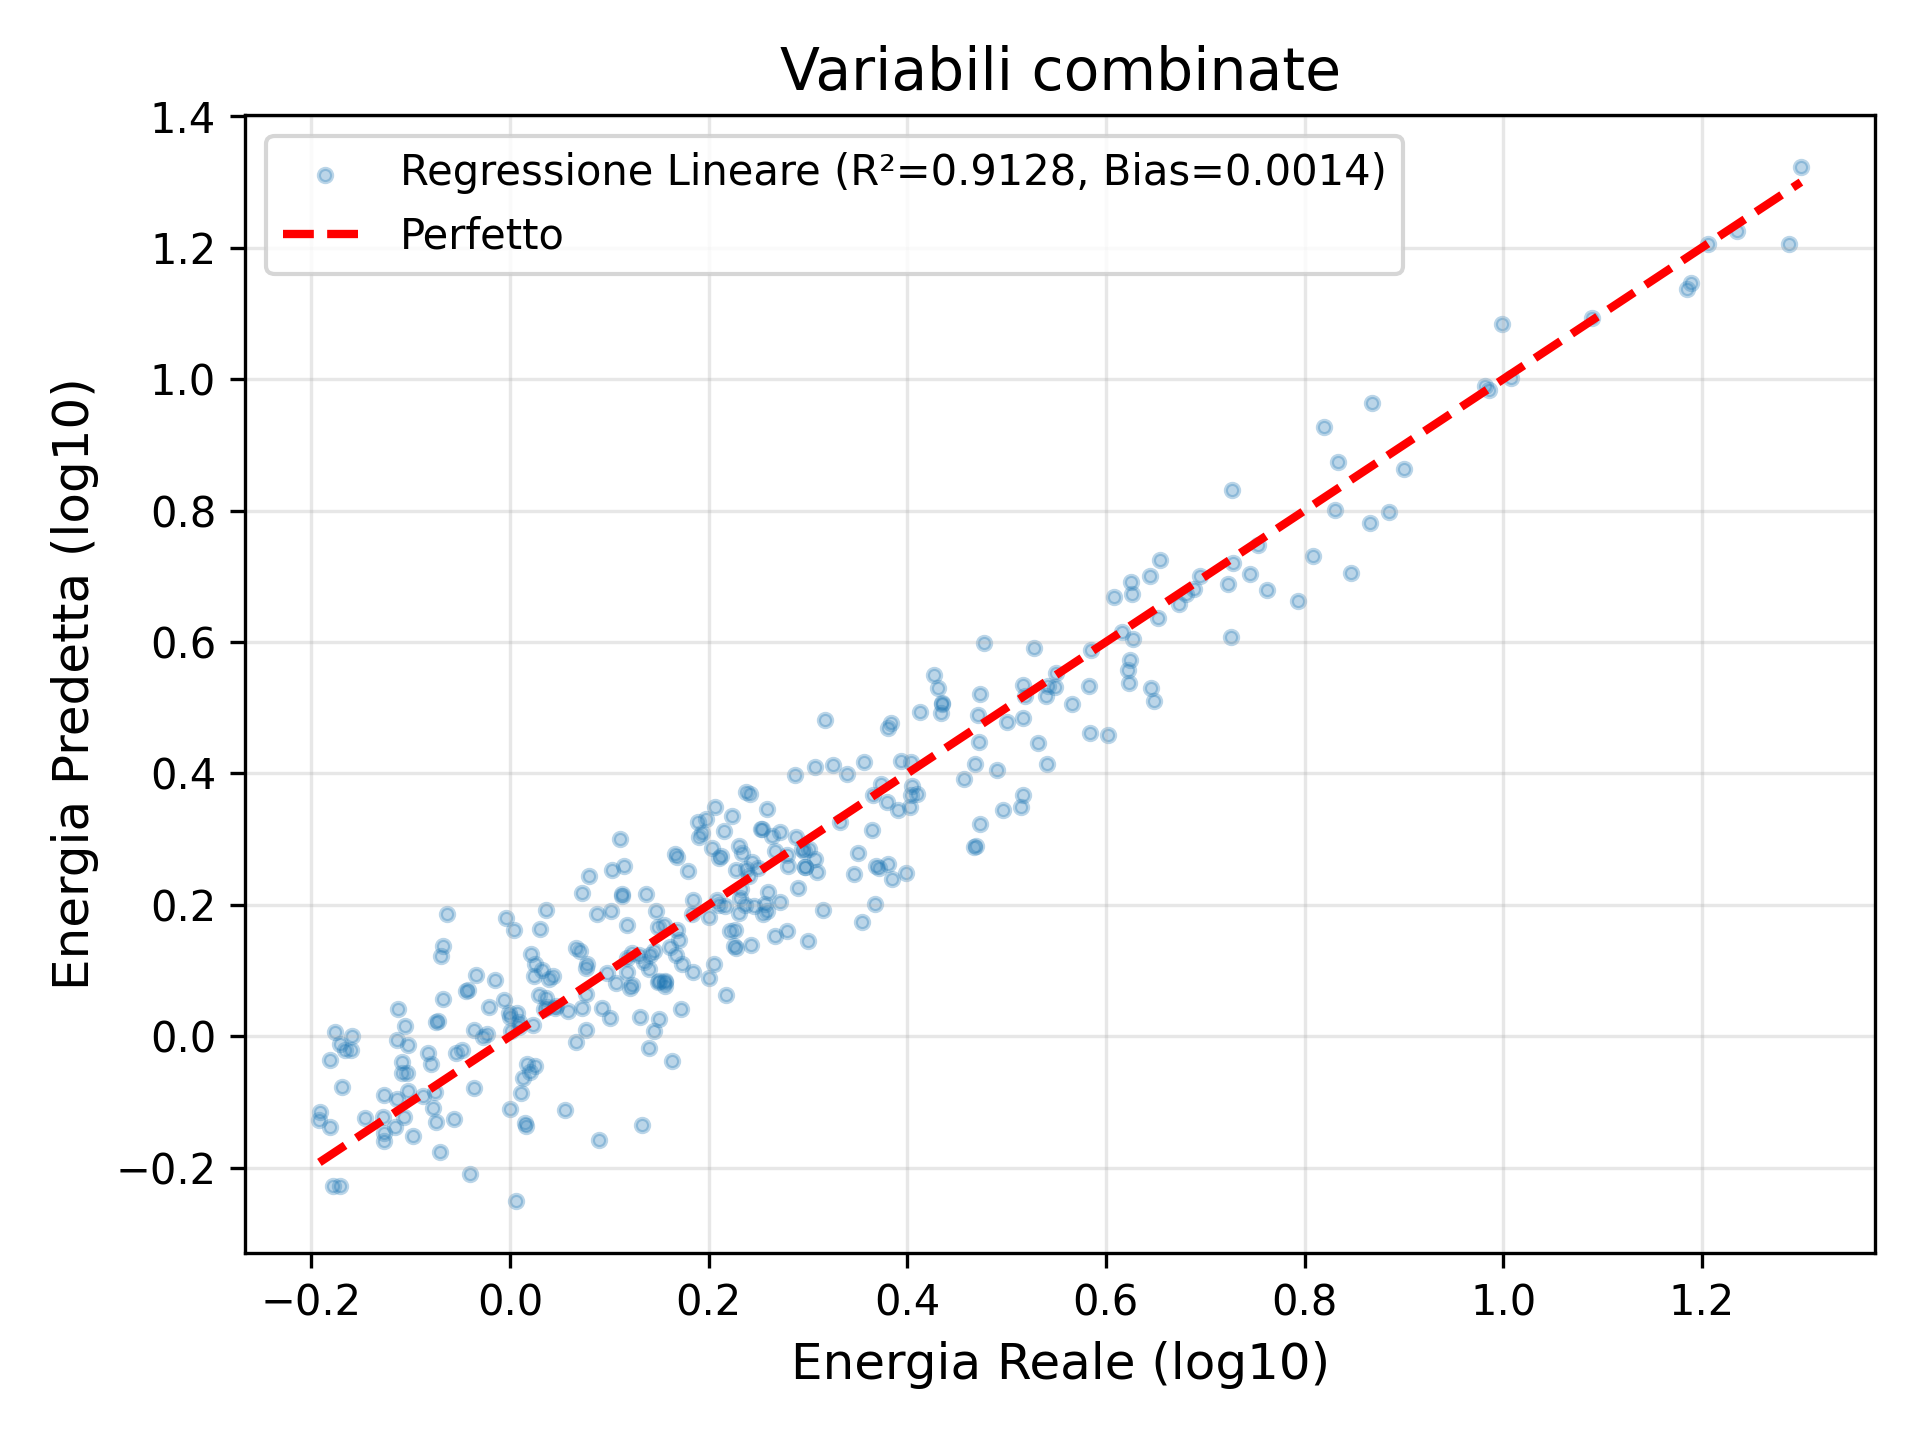
\includegraphics[width=0.5\textwidth]{CombVars.png}
\caption{Combinazione: manual + ing}
\label{default}
\end{center}
\end{figure}
Il risultato mostra un miglioramento notevole del $R^2$. La variabile principale resta sempre il segnale a terra, ma i contributi non lineari sembrano necessari, in particolare quelli legati alla forma della LDF. 
\end{frame}

\begin{frame}{Modelli Lineari - Grafico}
\begin{figure}[ht!]
\begin{center}
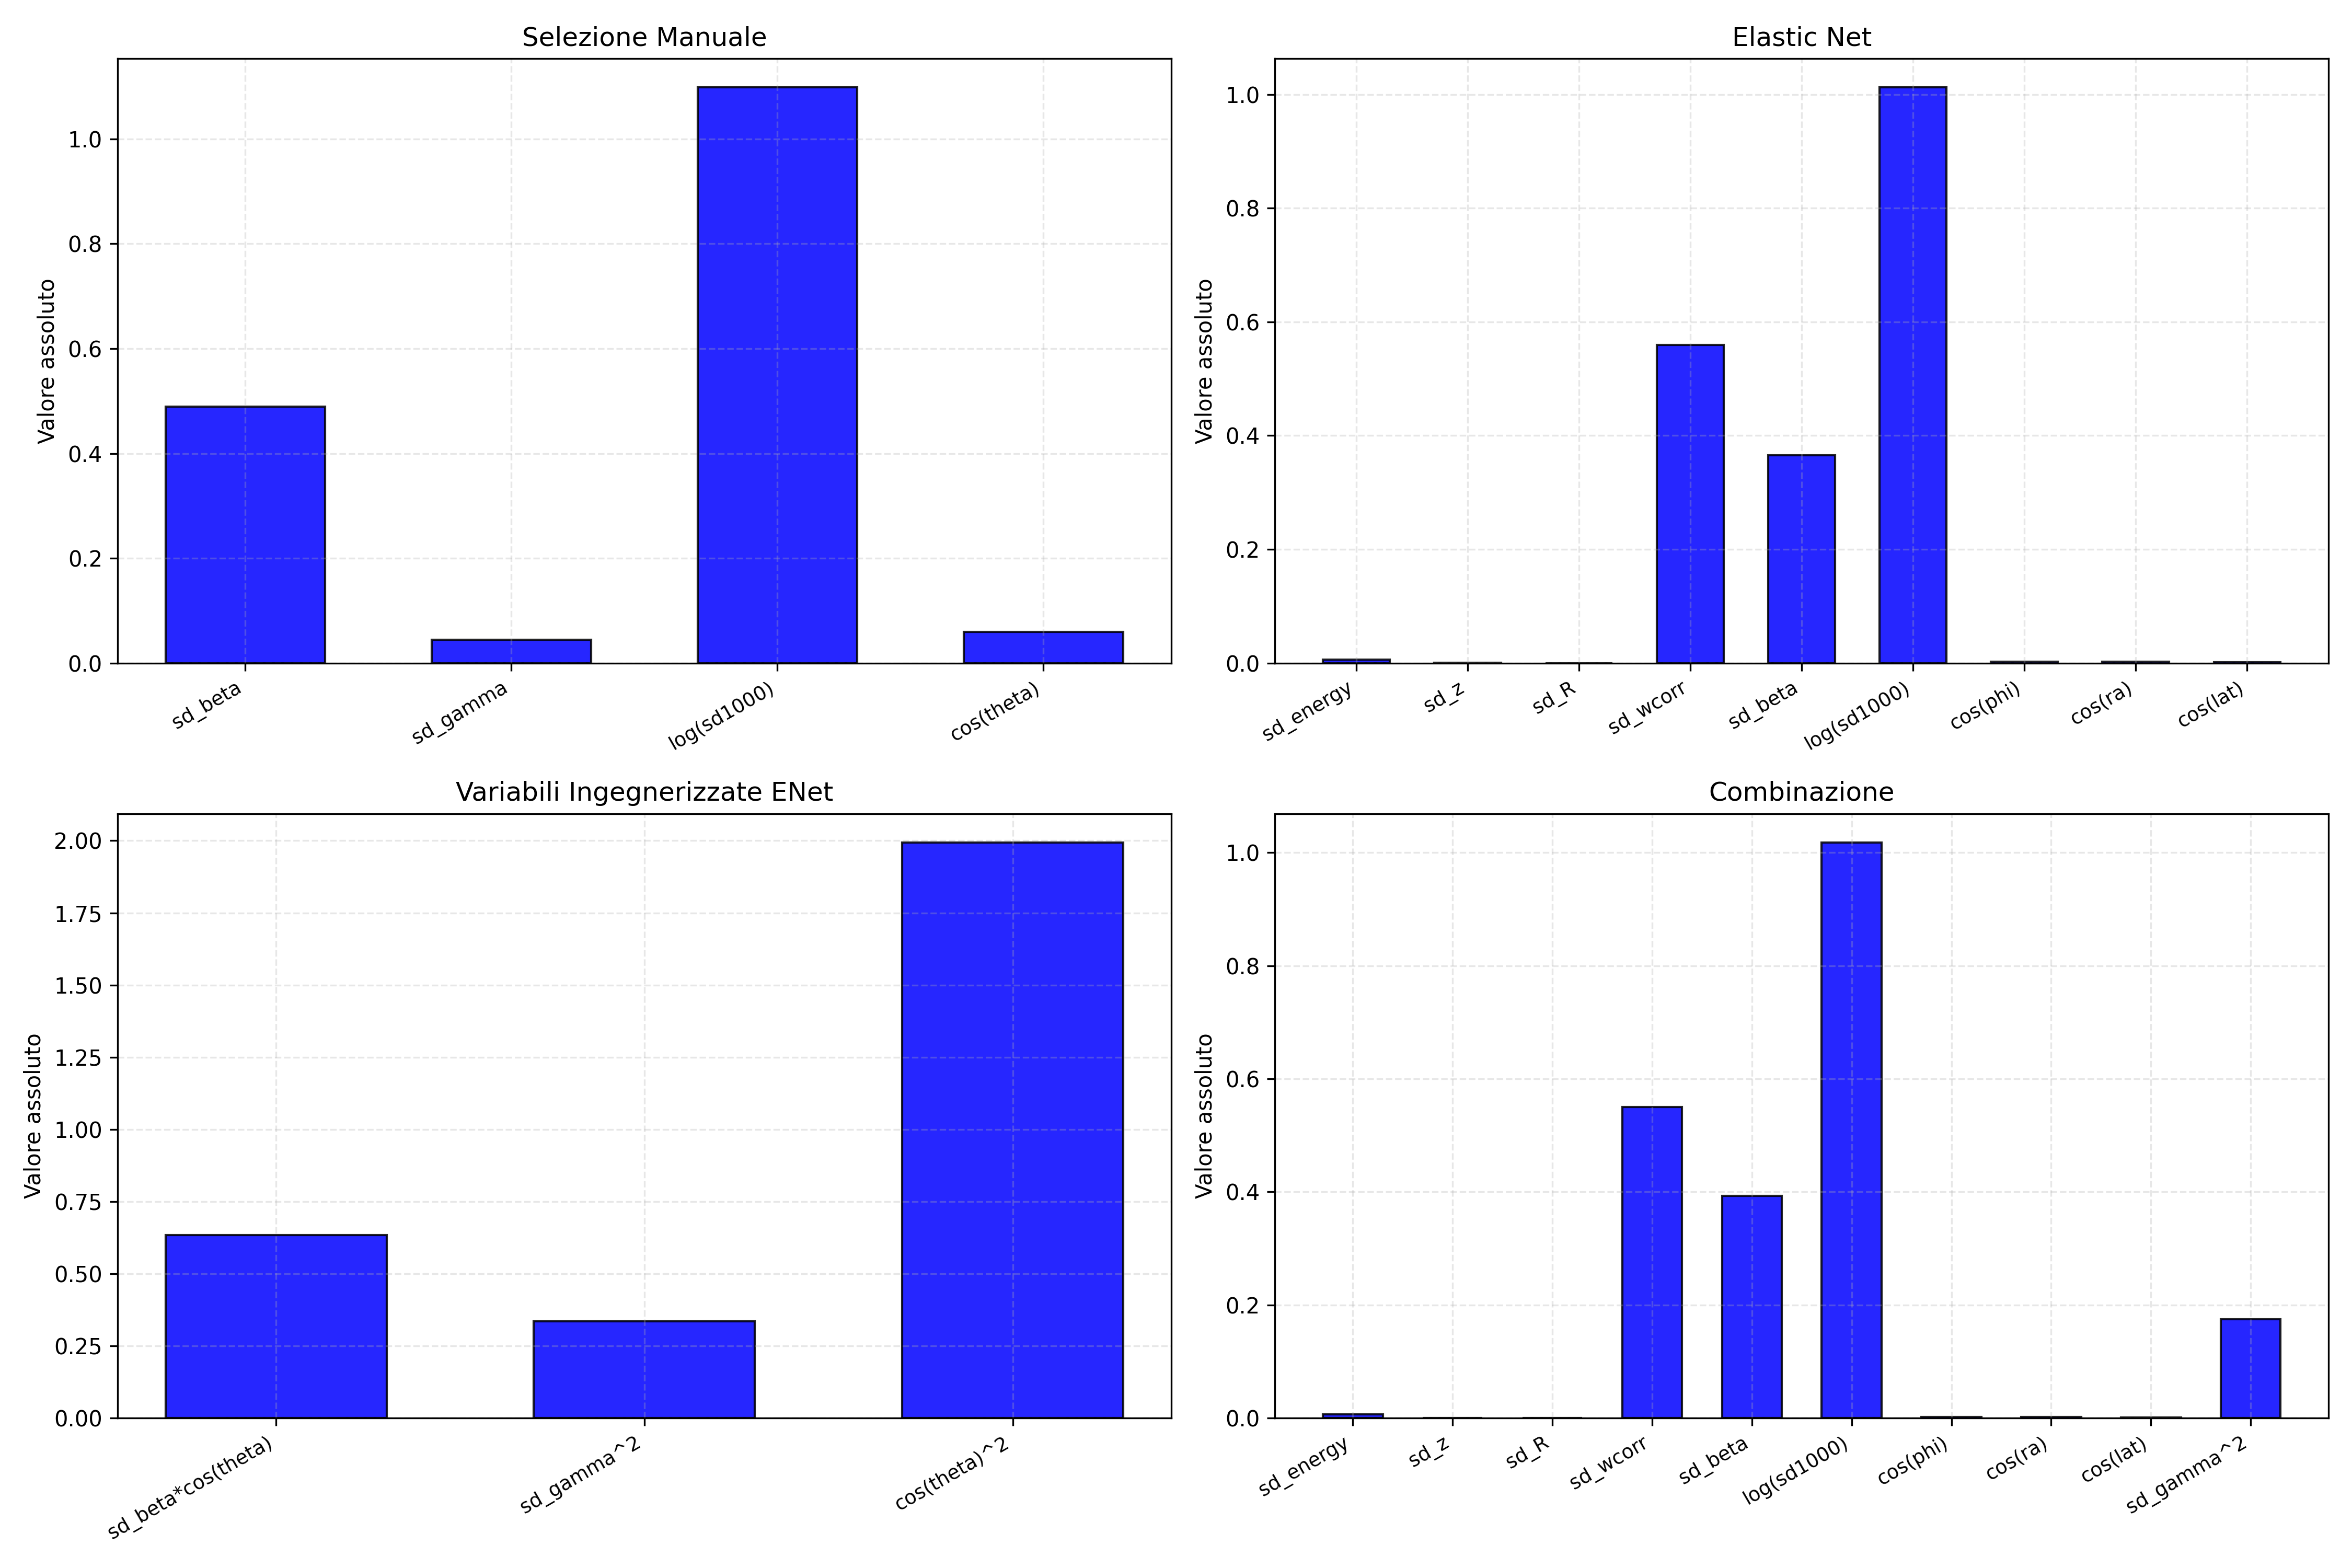
\includegraphics[width=0.85\textwidth]{Confronto_Coefficienti.png}
\caption{Riassunto dei Modelli Lineari}
\label{default}
\end{center}
\end{figure}
\end{frame}

\begin{frame}{Modelli Lineari }
Dai modelli lineari si capisce come il metodo CIC sia effettivamente valido, dato che la variabile principale è sempre il segnale a terra.\\ 
Non si possono escludere del tutto delle correzioni non lineari come suggerisce il modello a variabili ingegnerizzate.
\bigskip

Notiamo come nel modello combinato, le variabili ingegnerizzate abbiamo dei coefficienti elevati. Questo suggerisce che il loro contributo è piccolo ma esiste.
\bigskip

Il modello lineare è ovviamente la base d'appoggio per modelli più complessi (ML) ma cattura bene la fisica del problema. Il tutto può essere perfezionato attraverso strumenti più complessi, come si vede di seguito.
\end{frame}

\begin{frame}{Modelli Non Lineari}
La regressione lineare (anche con variabili ingegnerizzate) assume che le relazioni siano lineari o trasformabili. La fisica degli sciami potrebbe contenere effetti non lineari più complessi che un modello lineare non può catturare, motivo per cui si decide di procedere con dei modelli che superano questo ostacolo: gli \emph{ensemble methods} (EM).
\bigskip

L'obiettivo finale è correggere l'energia evento per evento. Se la correzione dipende da relazioni complesse tra morfologia, angolo e sviluppo dello sciame, un modello non lineare può catturarle meglio. Per questo progetto si è deciso di usare tre modelli diversi:
\begin{itemize}
\item \textcolor{blue}{Random Forest}.
\item \textcolor{blue}{Gradient Boosting}.
\item \textcolor{blue}{Extreme Gradient Boosting (XGB)}.
\end{itemize}
\end{frame}

\begin{frame}{Random Forest}
Il metodo Random Forest si basa sulla creazione di \emph{alberi decisionali} in parallelo, ognuno su un campione casuale dei dati (bootstrap) e su un sottoinsieme casuale delle variabili. La previsione finale è la media (per la regressione) dei risultati di tutti gli alberi.\\
È un metodo molto usato perché riduce la varianza del campione ed è "robusto" all'overfitting. 
\bigskip

Per testare il modello sono state usate sia le variabili scelte manualmente, sia le ristrette attraverso ENet. Inoltre, per verificare l'ipotesi di variabili ingegnerizzate, si è tentato di usare sia queste che la combinazione con le variabili lineari, al fine di osservare o meno un miglioramento del modello.
\end{frame}

\begin{frame}{Random Forest - Grafico}
\begin{figure}[ht!]
\begin{center}
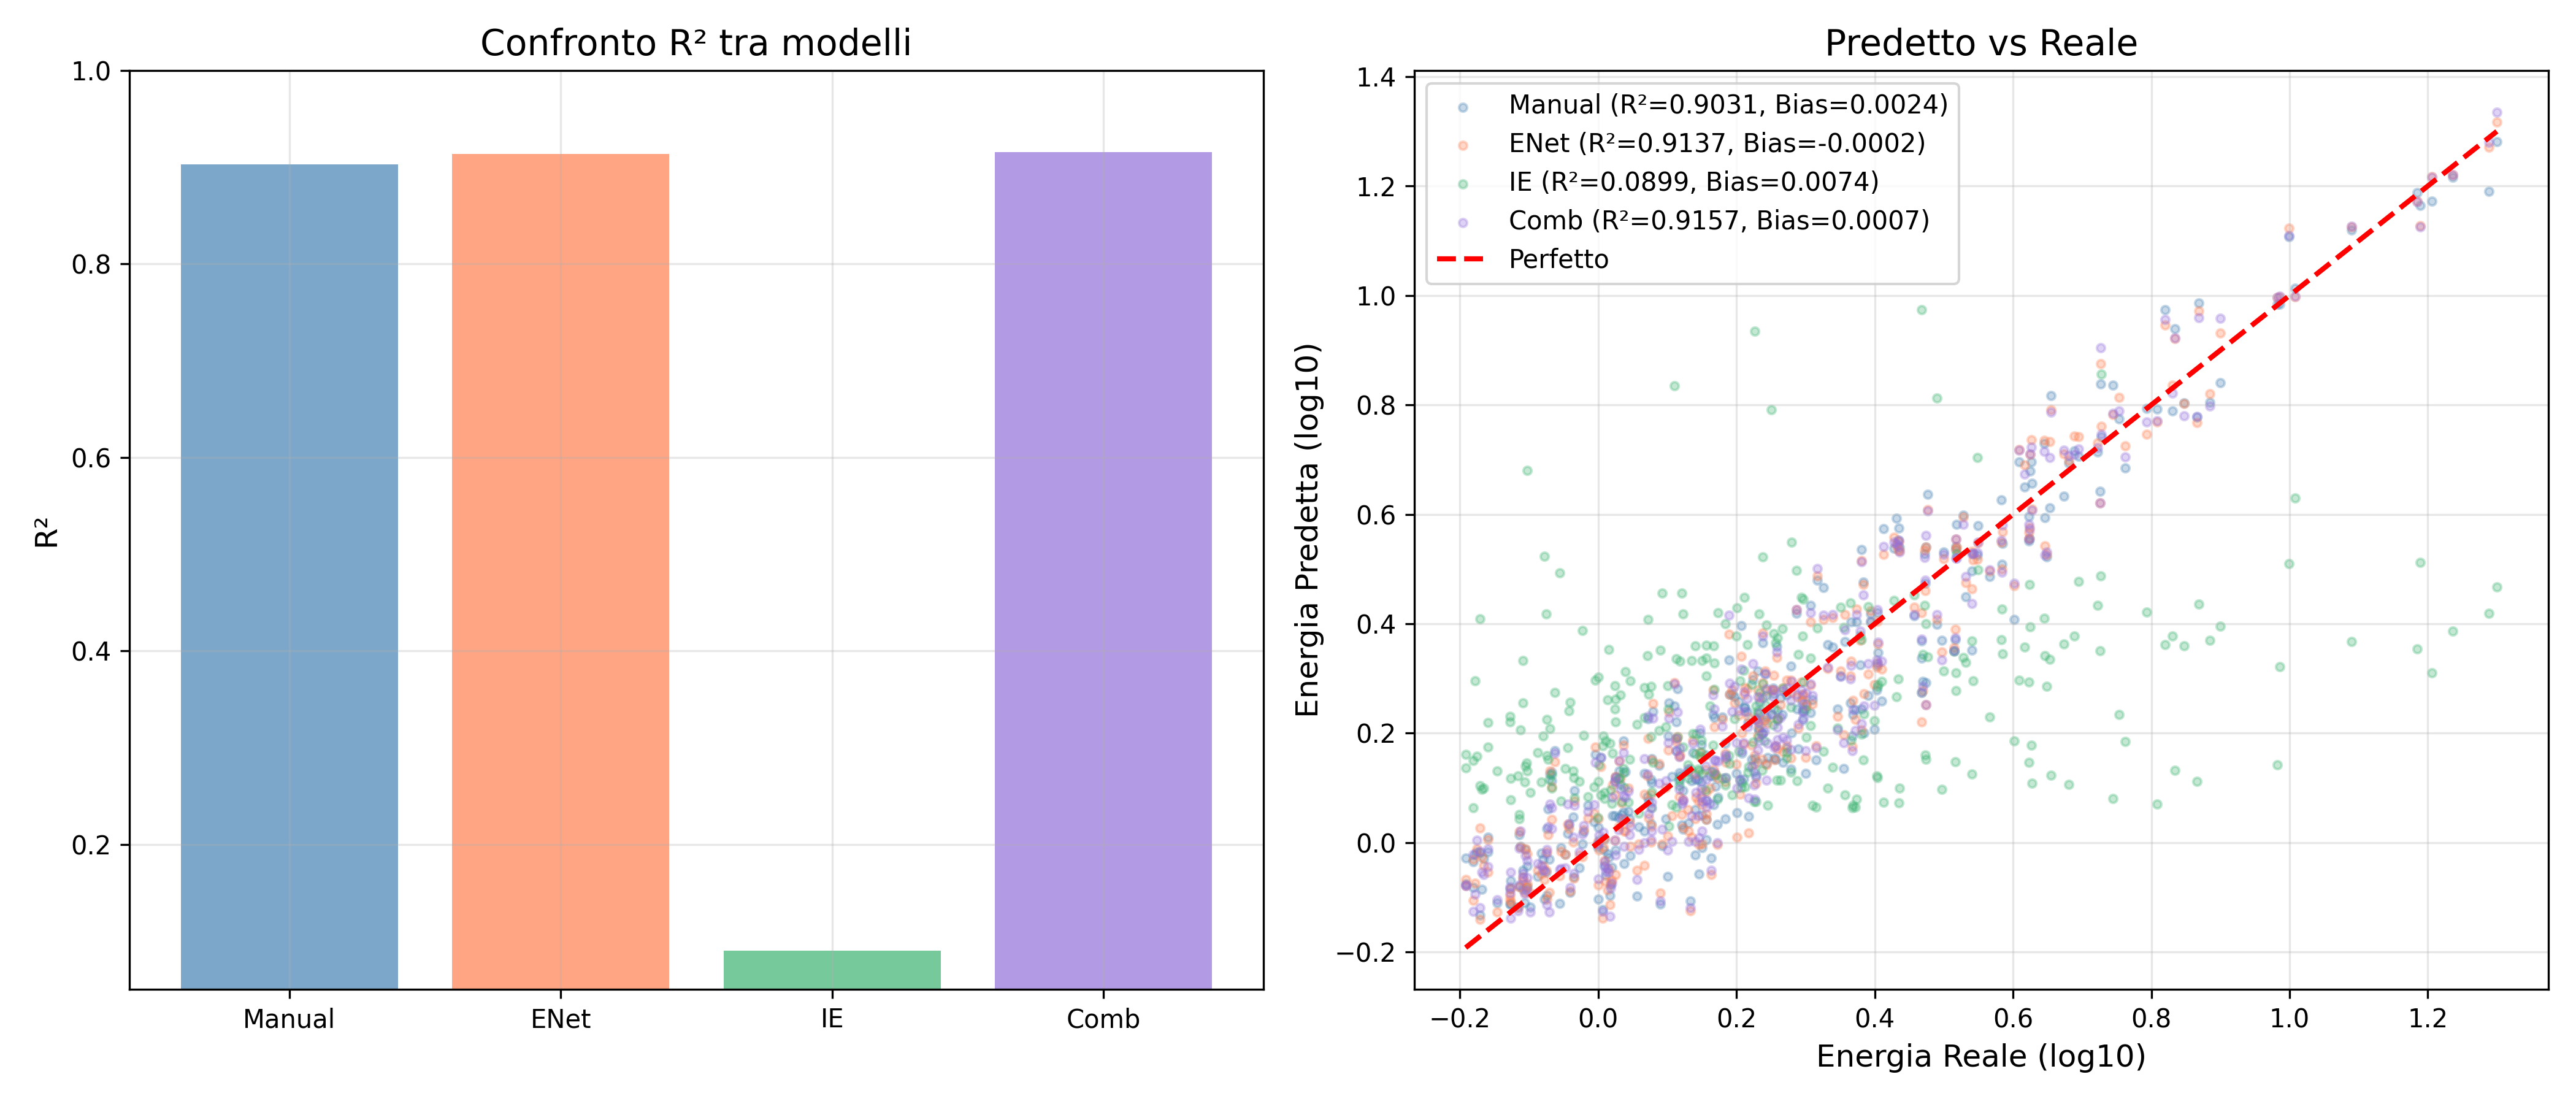
\includegraphics[width = 0.8 \textwidth]{RF_Confronto.png}
\caption{Confronto tra i fit di Random Forest}
\label{default}
\end{center}
\end{figure}
Dal grafico si evince che il modello migliore per Random Forest è quello a variabili scelte manualmente. Gli altri fit sono leggermente peggiori rispetto ai corrispettivi lineari, suggerendo che la relazione lineare cattura gran parte della fisica rilevante. 
\end{frame}

\begin{frame}{Gradient Boosting}
Il metodo Gradient Boosting si basa sulla creazione di \emph{alberi decisionali} in sequenza, facendo si che ogni albero corregga gli errori del precedente. Il tutto si basa sul seguire il gradiente della \emph{funzione di perdita}. Il risultato è un modello altamente preciso, in grado di catturare interazioni complesse.
\bigskip

Per testare il modello sono state usate le stesse variabili del Random Forest, per verificare miglioramenti rispetto ai modelli lineari o al Random Forest stesso.
\end{frame}
\begin{frame}{Gradient Boosting - Grafico}
\begin{figure}[ht!]
\begin{center}
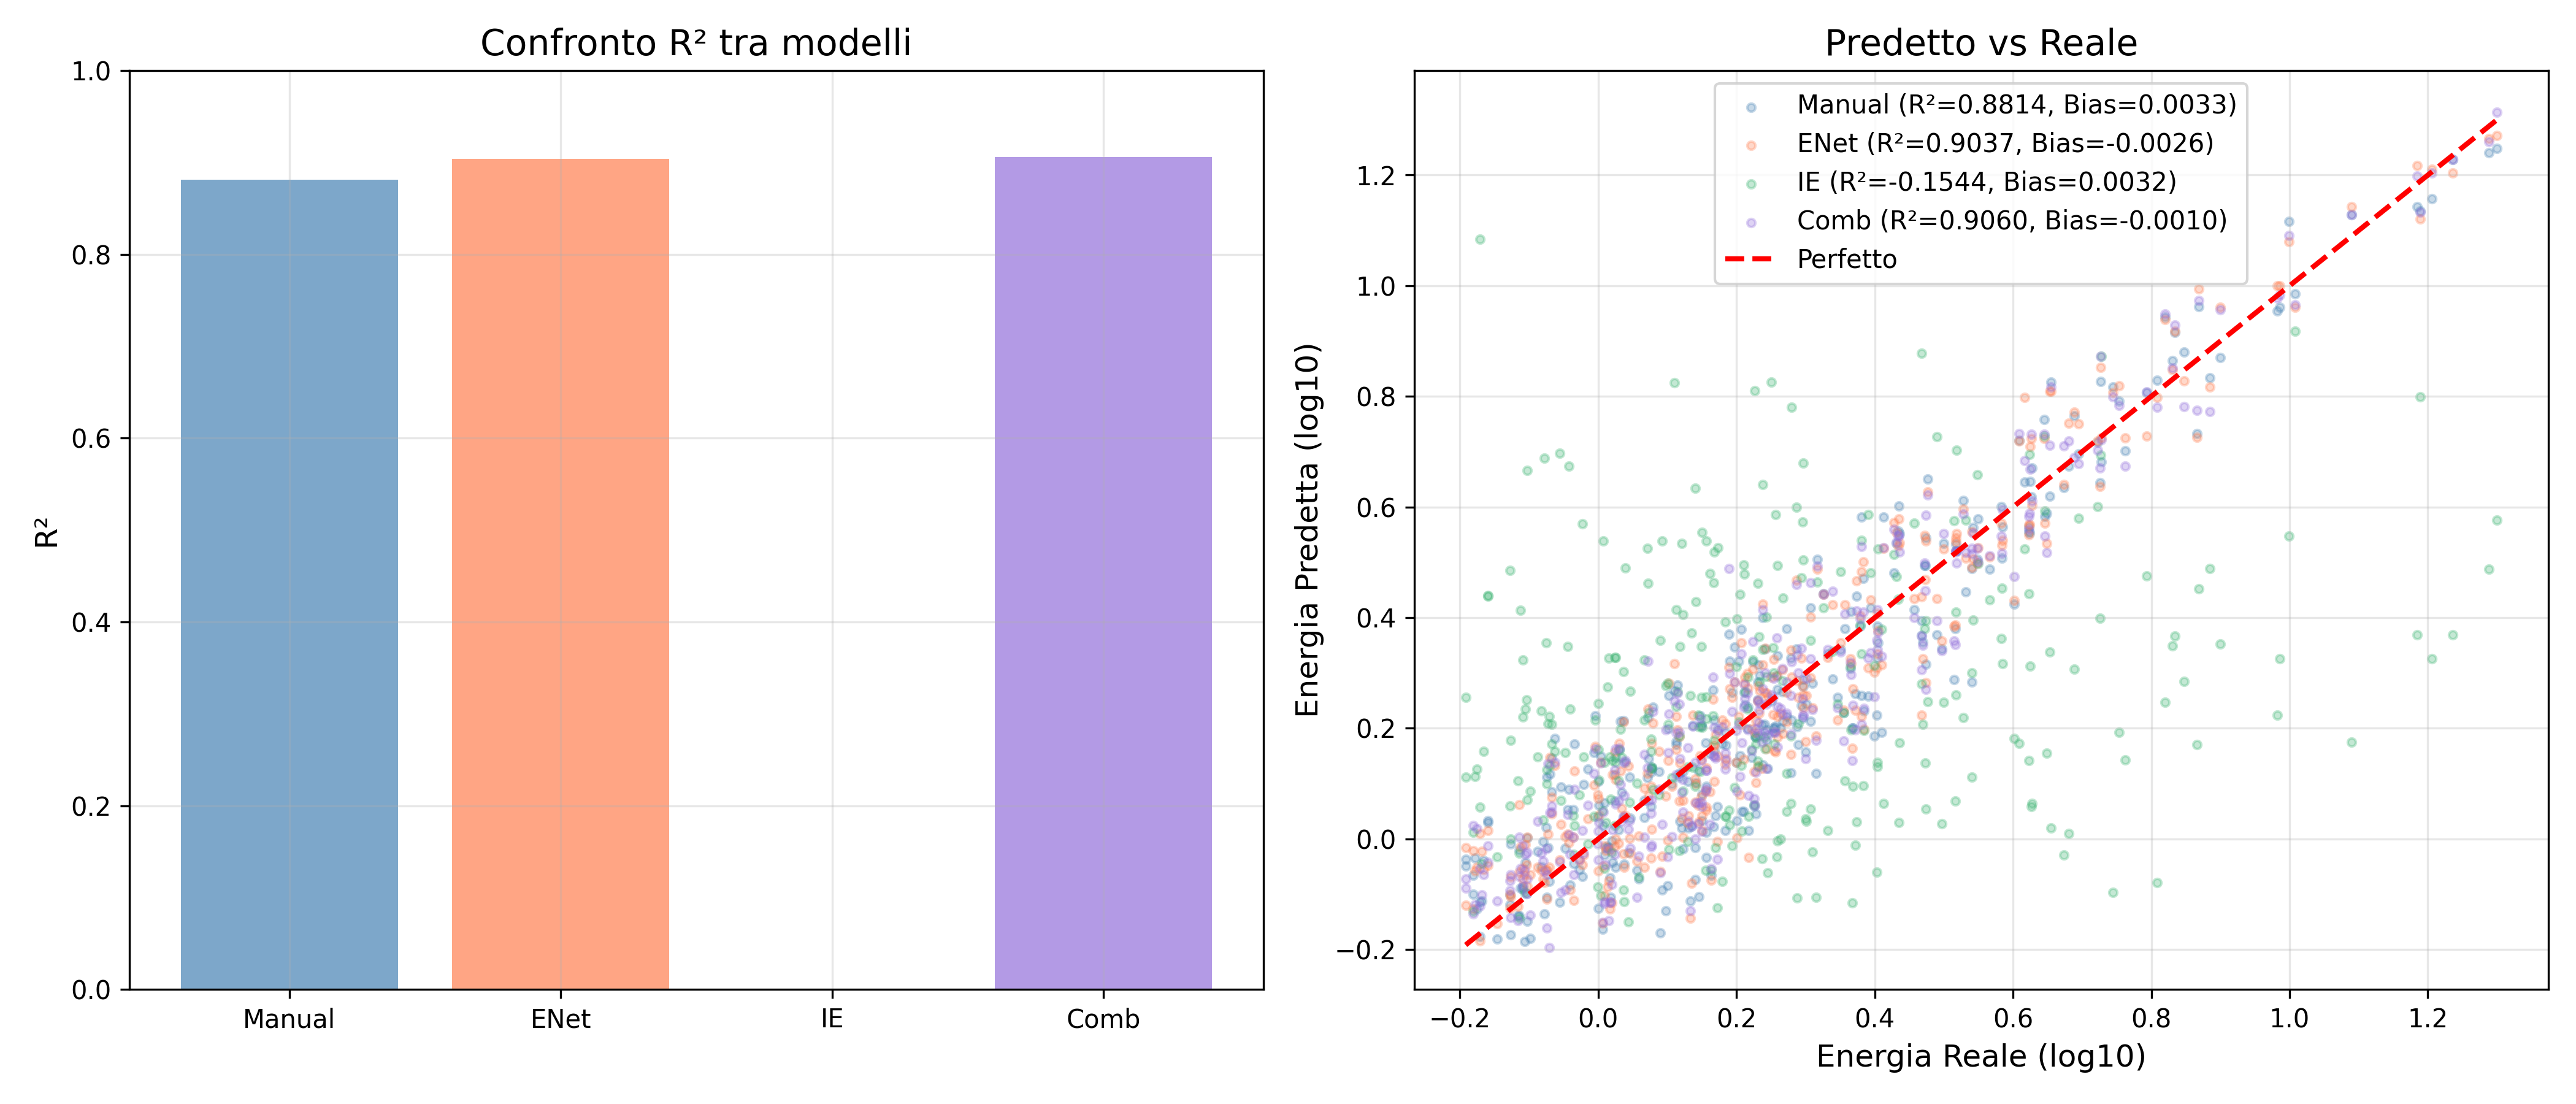
\includegraphics[width = 0.75 \textwidth]{GB_Confronto.png}
\caption{Confronto tra i fit di Gradient Boosting}
\label{default}
\end{center}
\end{figure}
Dal grafico si evince che il modello migliore per Gradient Boosting è quello a variabili scelte manualmente. Si può notare un miglioramento rispetto a Random Forest, eccetto per le variabili combinate (modello non buono). L'indice $R^2$ per ENet raggiunge quasi i livelli della regressione lineare, ma il fatto che sia minore suggerisce che ci sia della correlazione che influisce sul risultato.
\end{frame}

\begin{frame}{XGB}
Il metodo XGB è una versione migliorata del Gradiente Boosting. Il principio di funzionamento è lo stesso, ma si aggiunge una regolarizzazione simile ad ENet per ridurre l'overfitting. Questa regolarizzazione è accompagnata da una sorta di "potatura" nel caso di alberi complessi che non portano a miglioramenti e da una doppia derivazione (gradiente ed Hessiano). Il tutto rende il modello più veloce ed efficiente.
\bigskip

Il motivo principale per usare XGB in questo caso è verificare se il dataset presenta delle criticità tali da rendere questo modello più valido del normale Gradient Boosting.
\end{frame}
\begin{frame}{XGB - Grafico}
\begin{figure}[ht!]
\begin{center}
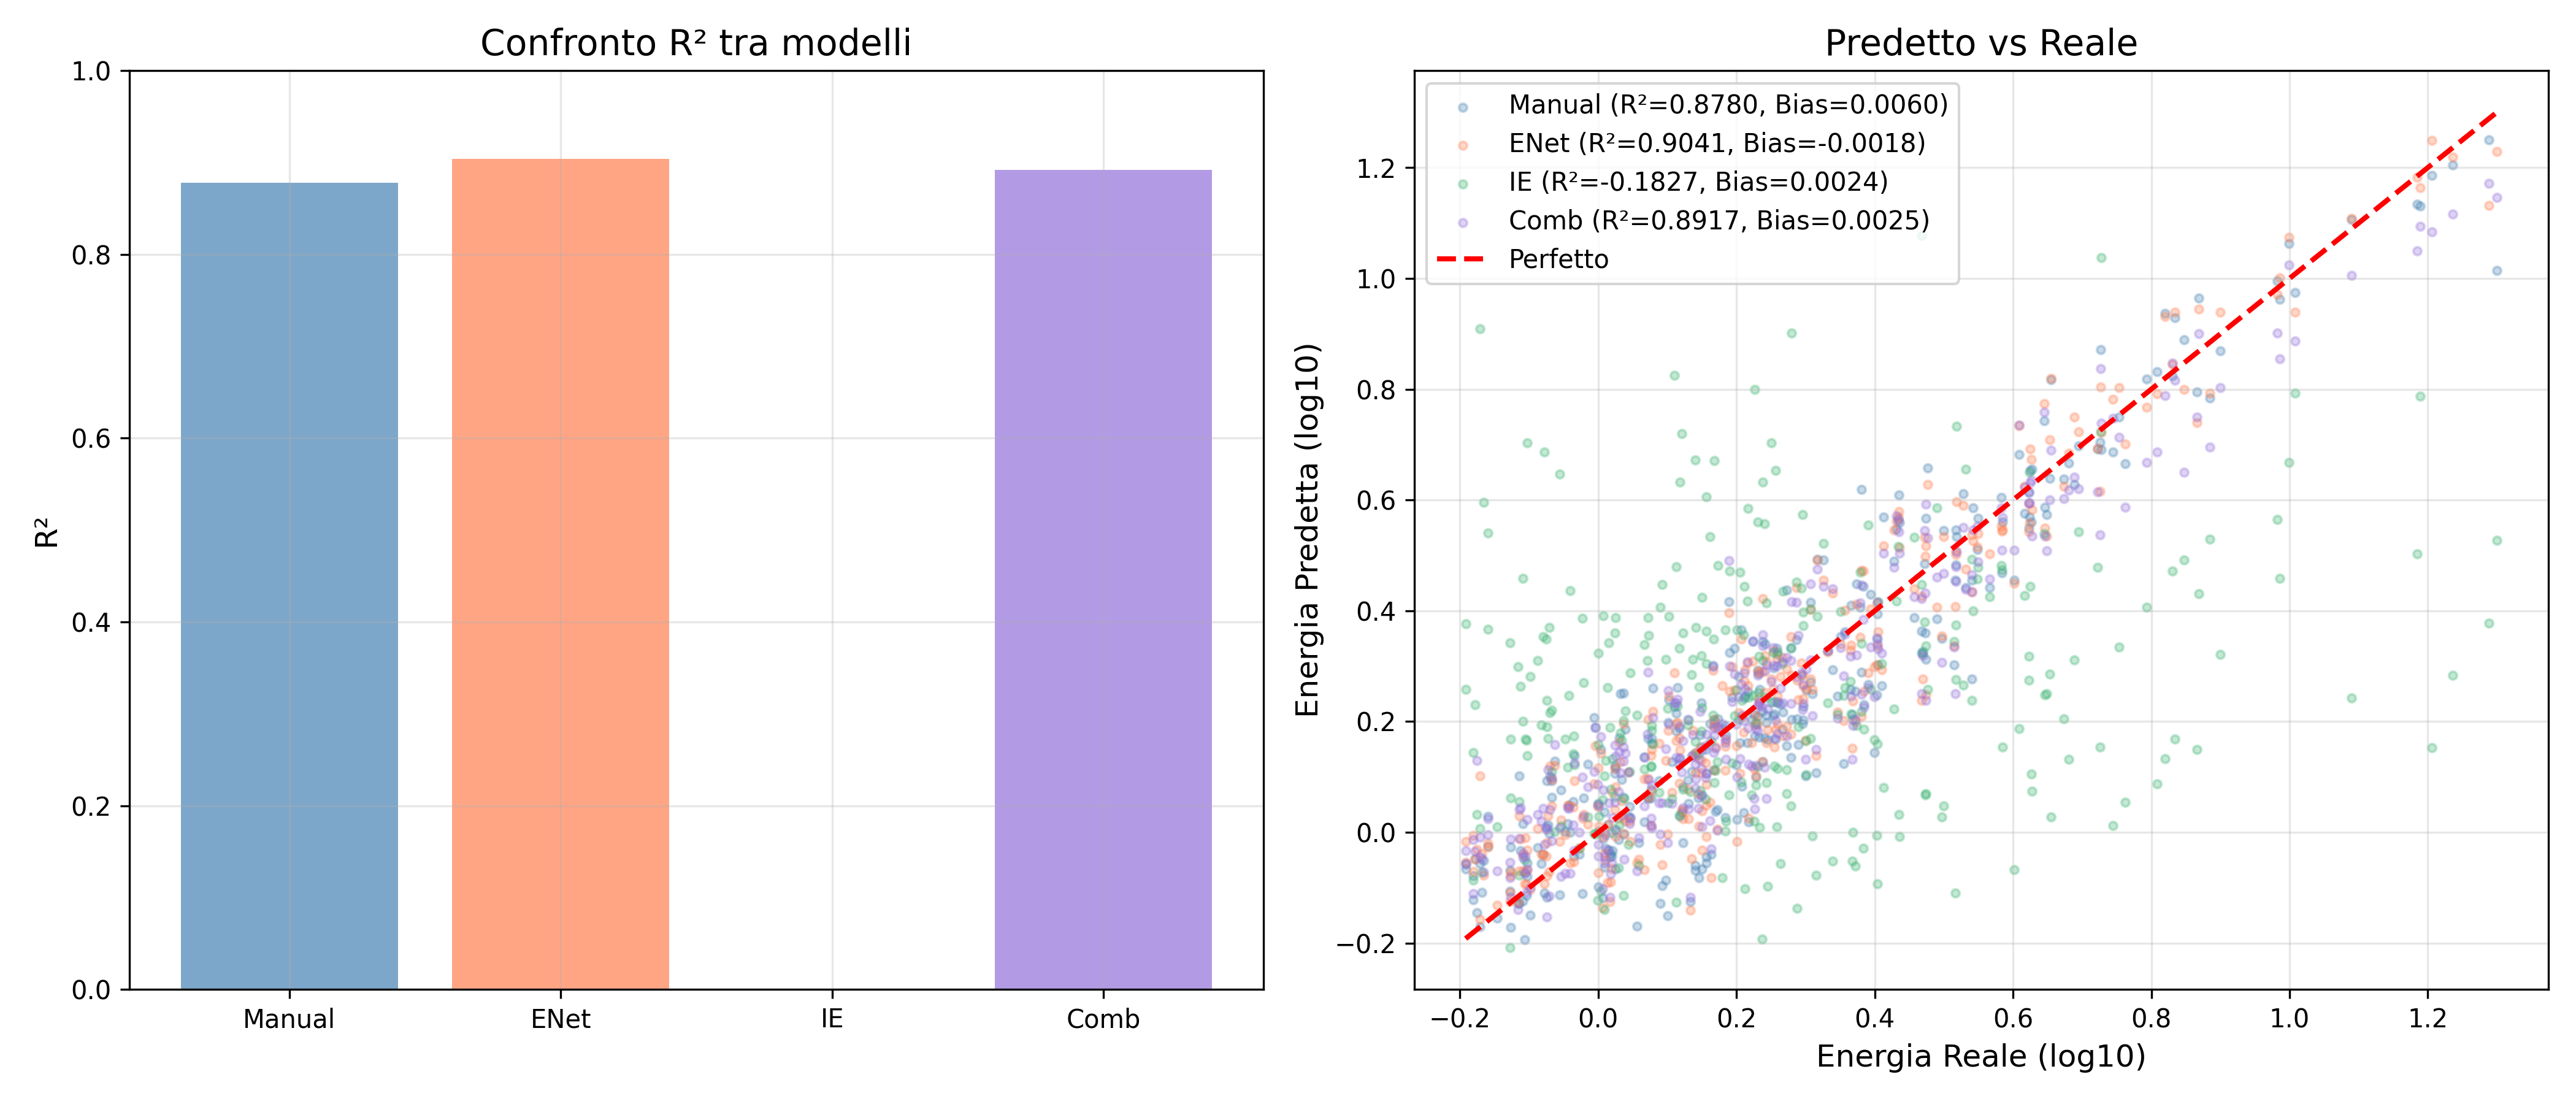
\includegraphics[width = 0.75 \textwidth]{XGB_Confronto.png}
\caption{Confronto tra i fit di XGB}
\label{default}
\end{center}
\end{figure}
Dal grafico si evince che il modello migliore per XGB è quello a variabili scelte manualmente. Gli indici $R^2$ leggermente minori suggeriscono che il dataset non presenta criticità e che Gradient Boosting basta e avanza per osservare relazioni tra le variabili scelte.
\end{frame}

\begin{frame}{Metodi Ensemble - Grafico}
\begin{figure}[t!]
\begin{center}
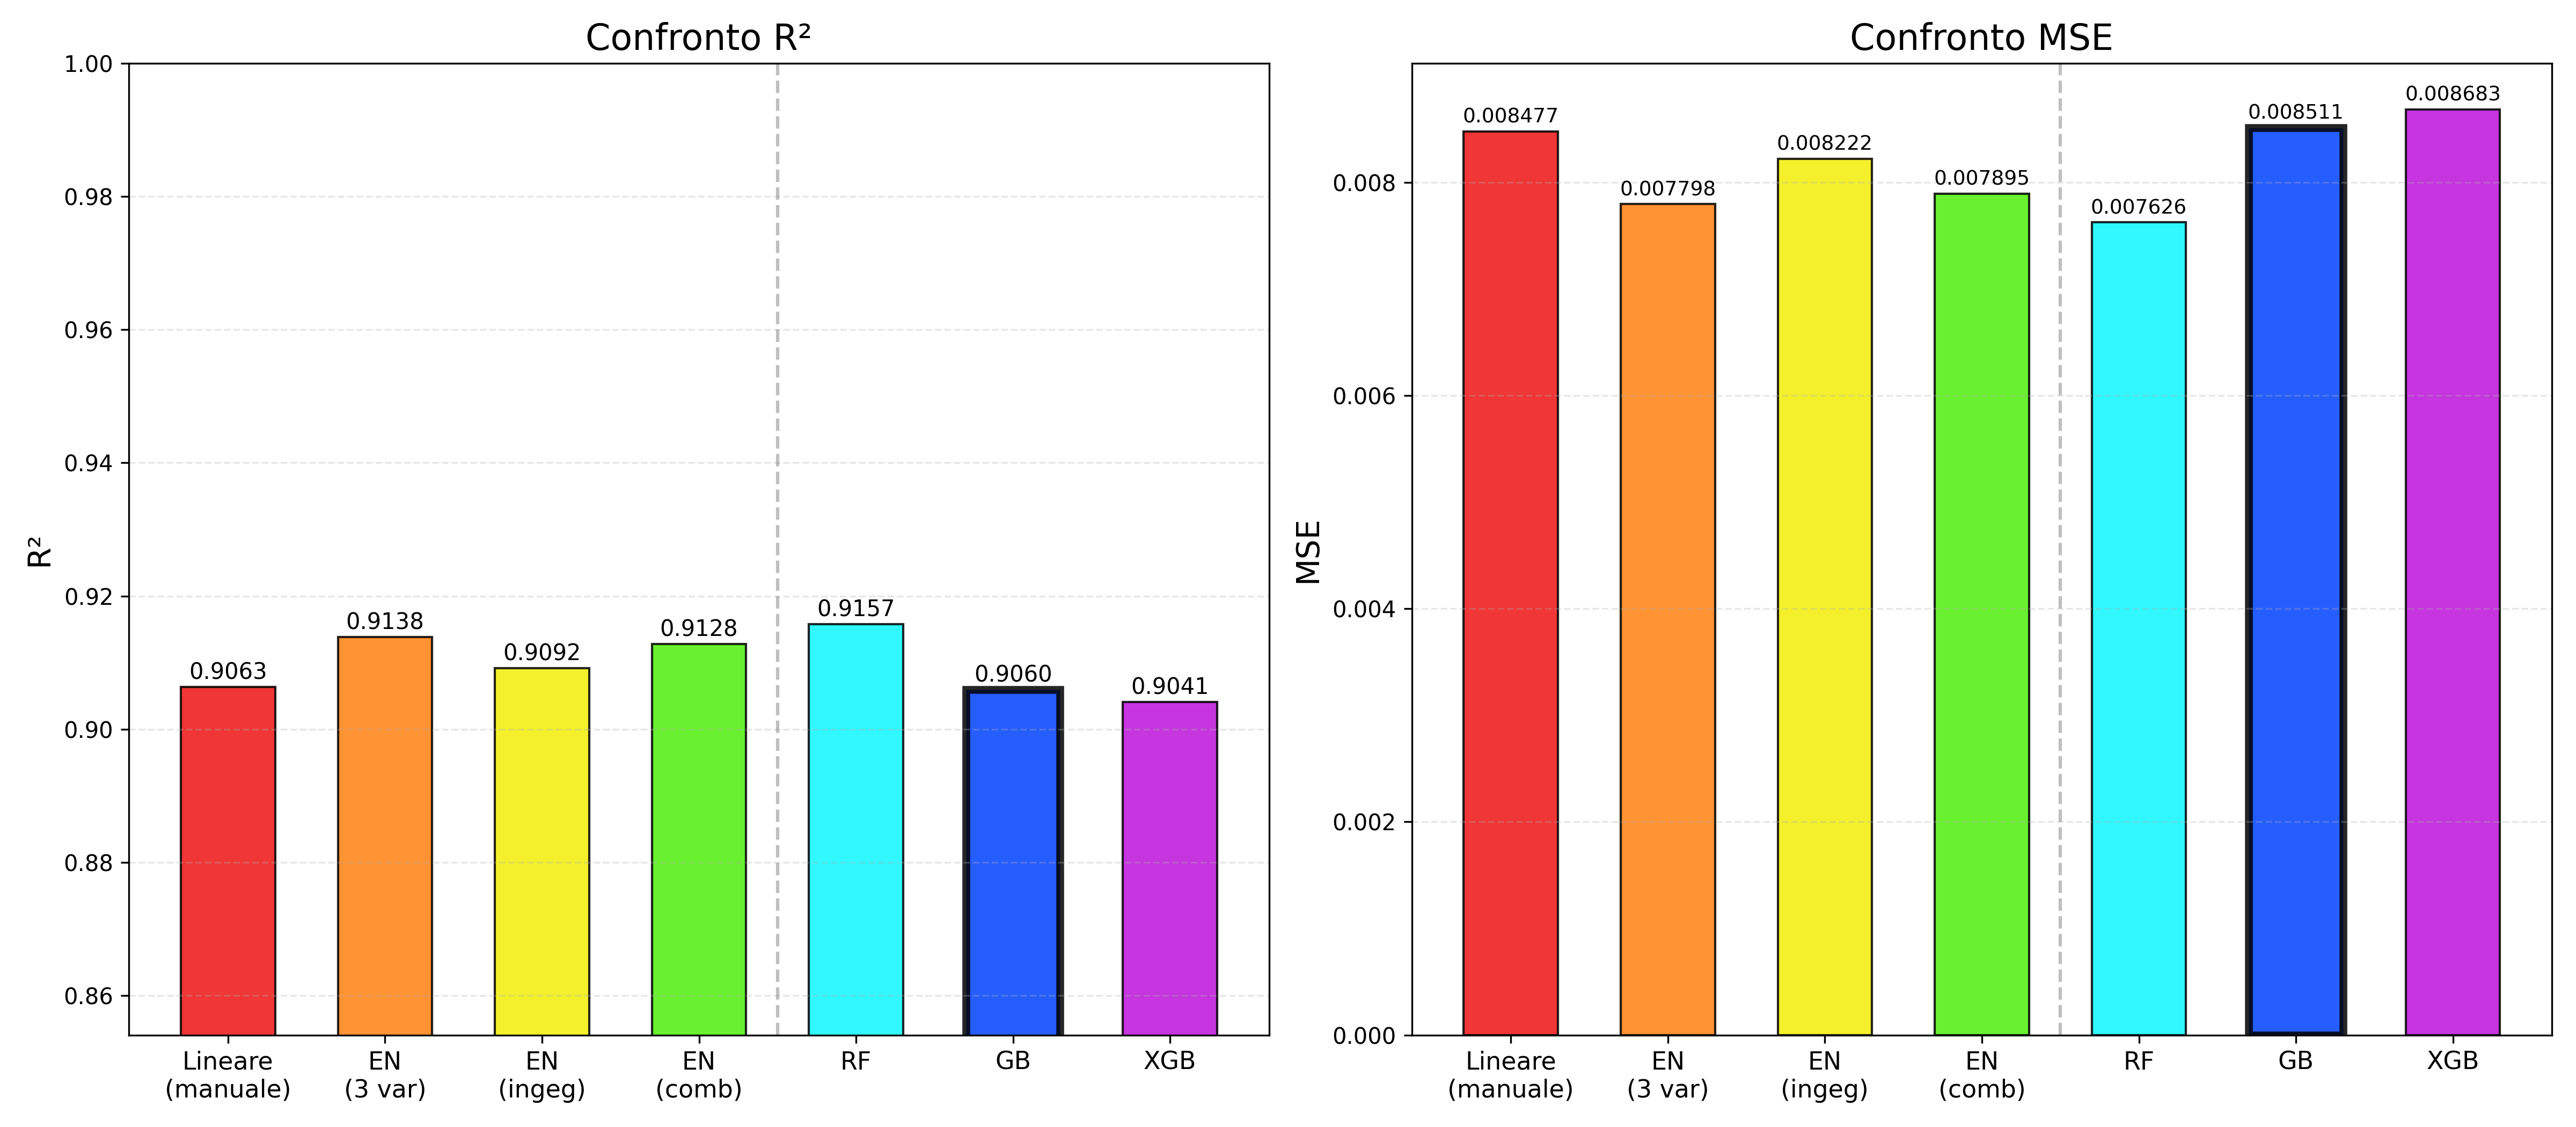
\includegraphics[width=\textwidth]{Confronto_R2_MSE.png}
\caption{Risultati dei fit nei Metodi Ensemble}
\label{default}
\end{center}
\end{figure}
Dalla figura si evince il miglioramento dei metodi di ensemble rispetto alla regressione lineare, sia come aumento di $R^2$ che come diminuzione dello scarto quadratico medio (MSE).
\end{frame}

\begin{frame}{Importanza delle Variabili}
\begin{figure}[htbp]
\begin{center}
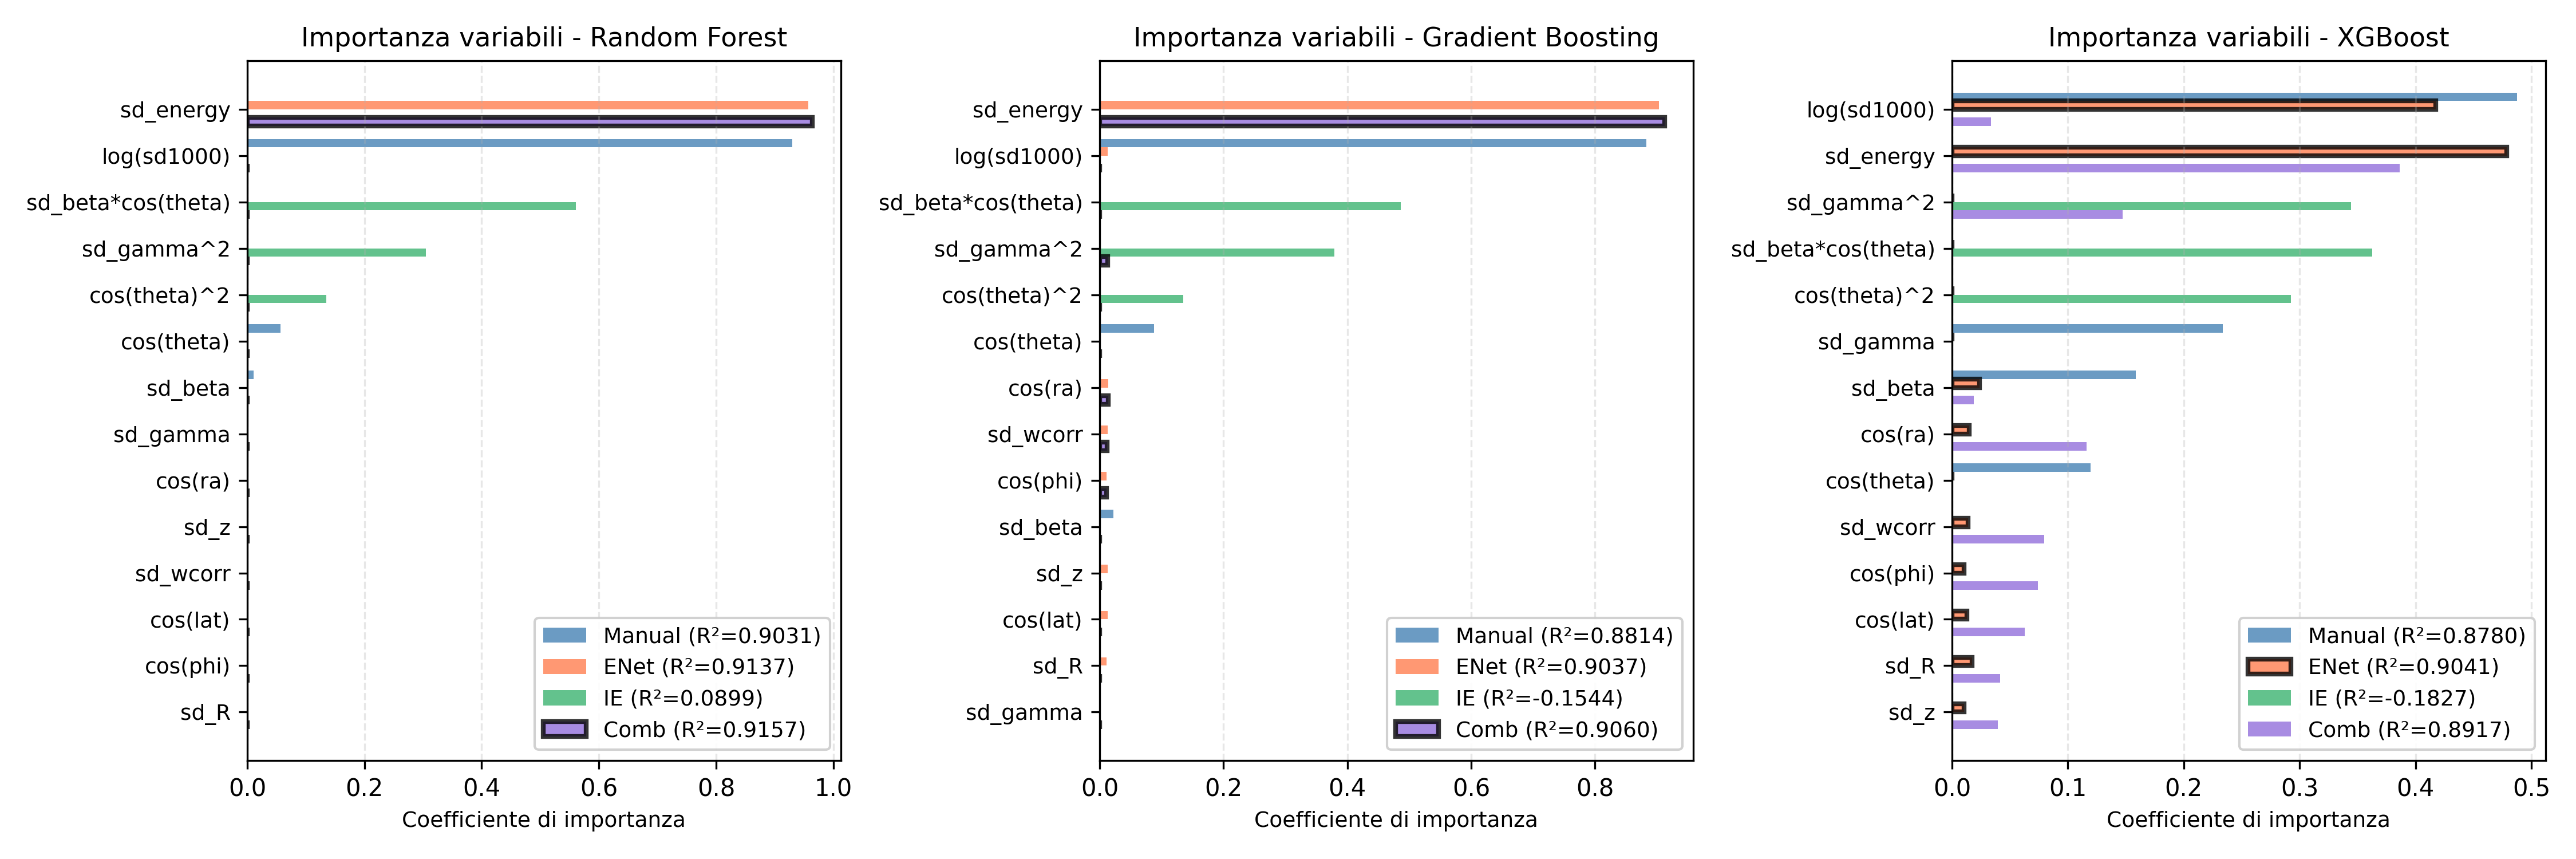
\includegraphics[width=\textwidth]{Confronto_Importanza_Variabili.png}
\caption{Confronto di importanza variabili}
\label{default}
\end{center}
\end{figure}
Dal seguente grafico possiamo dedurre che la variabile fondamentale per ricostruire l'energia è sempre il segnale a terra. Rispetto a quanto suggeriscono i modelli lineari, l'altro contributo principale lo fornisce l'angolo zenitale. Fa eccezione XGB che invece mette quasi sullo stesso piano il segnale e la forma della LDF, per poi usare $\beta, \cos(\theta)$ per meno del 5\%.
\end{frame}

\begin{frame}{Conclusioni}
Dall'analisi di tutti i modelli possiamo trarre conclusioni interessanti:
\begin{itemize}
    \item La regressione lineare, con le variabili selezionate manualmente, coglie già la fisica fondamentale alla base della ricostruzione dell'energia. Il miglioramento ottenuto con le variabili ingegnerizzate non introduce nuova fisica, ma suggerisce la presenza di relazioni non lineari che un modello lineare non può catturare appieno.
    \item Random Forest migliora la regressione lineare, confermando le ipotesi precedenti e dimostrando che le non-linearità suggerite sono effettivamente presenti nei dati. Il modello basato su variabili selezionate secondo la conoscenza fisica risulta il più valido.
    \item Gradient Boosting supera tutti gli altri metodi, raggiungendo le prestazioni migliori in modo coerente con le aspettative. 
    \item XGBoost non ha prodotto ulteriori miglioramenti significativi rispetto a Gradient Boosting. Questo risultato suggerisce che il dataset è ben pulito e che le relazioni fisiche sono già state completamente catturate.
\end{itemize}
\end{frame}

\begin{frame}{Ultimo confronto}
La verifica finale l'efficacia del modello di Machine Learning rispetto al metodo standard CIC si può osservare confrontando una calibrazione CIC sugli eventi \emph{golden hybrids} con il modello Gradient Boosting con variabili selezionate manualmente.
\bigskip

La scelta degli eventi golden deriva dal fatto che in questi sono gli unici eventi per i quali è disponibile l'energia misurata da FD, che rappresenta la "verità" indipendente necessaria per validare la ricostruzione.
\bigskip

Il modello Gradient Boosting mostra un R² del 99.78\% sui dati di training, ma scende al 90.14\% se applicato ai golden hybrids. Questo calo, pur significativo, è fisiologico: il modello è stato addestrato su un target proxy (l'energia CIC) e validato su un target indipendente (l'energia FD). La differenza riflette la discrepanza tra la ricostruzione CIC e la misura FD, che il modello cerca di correggere. Il tutto si osserva nella slide seguente
\end{frame}

\begin{frame}
\begin{figure}[htbp]
\begin{center}
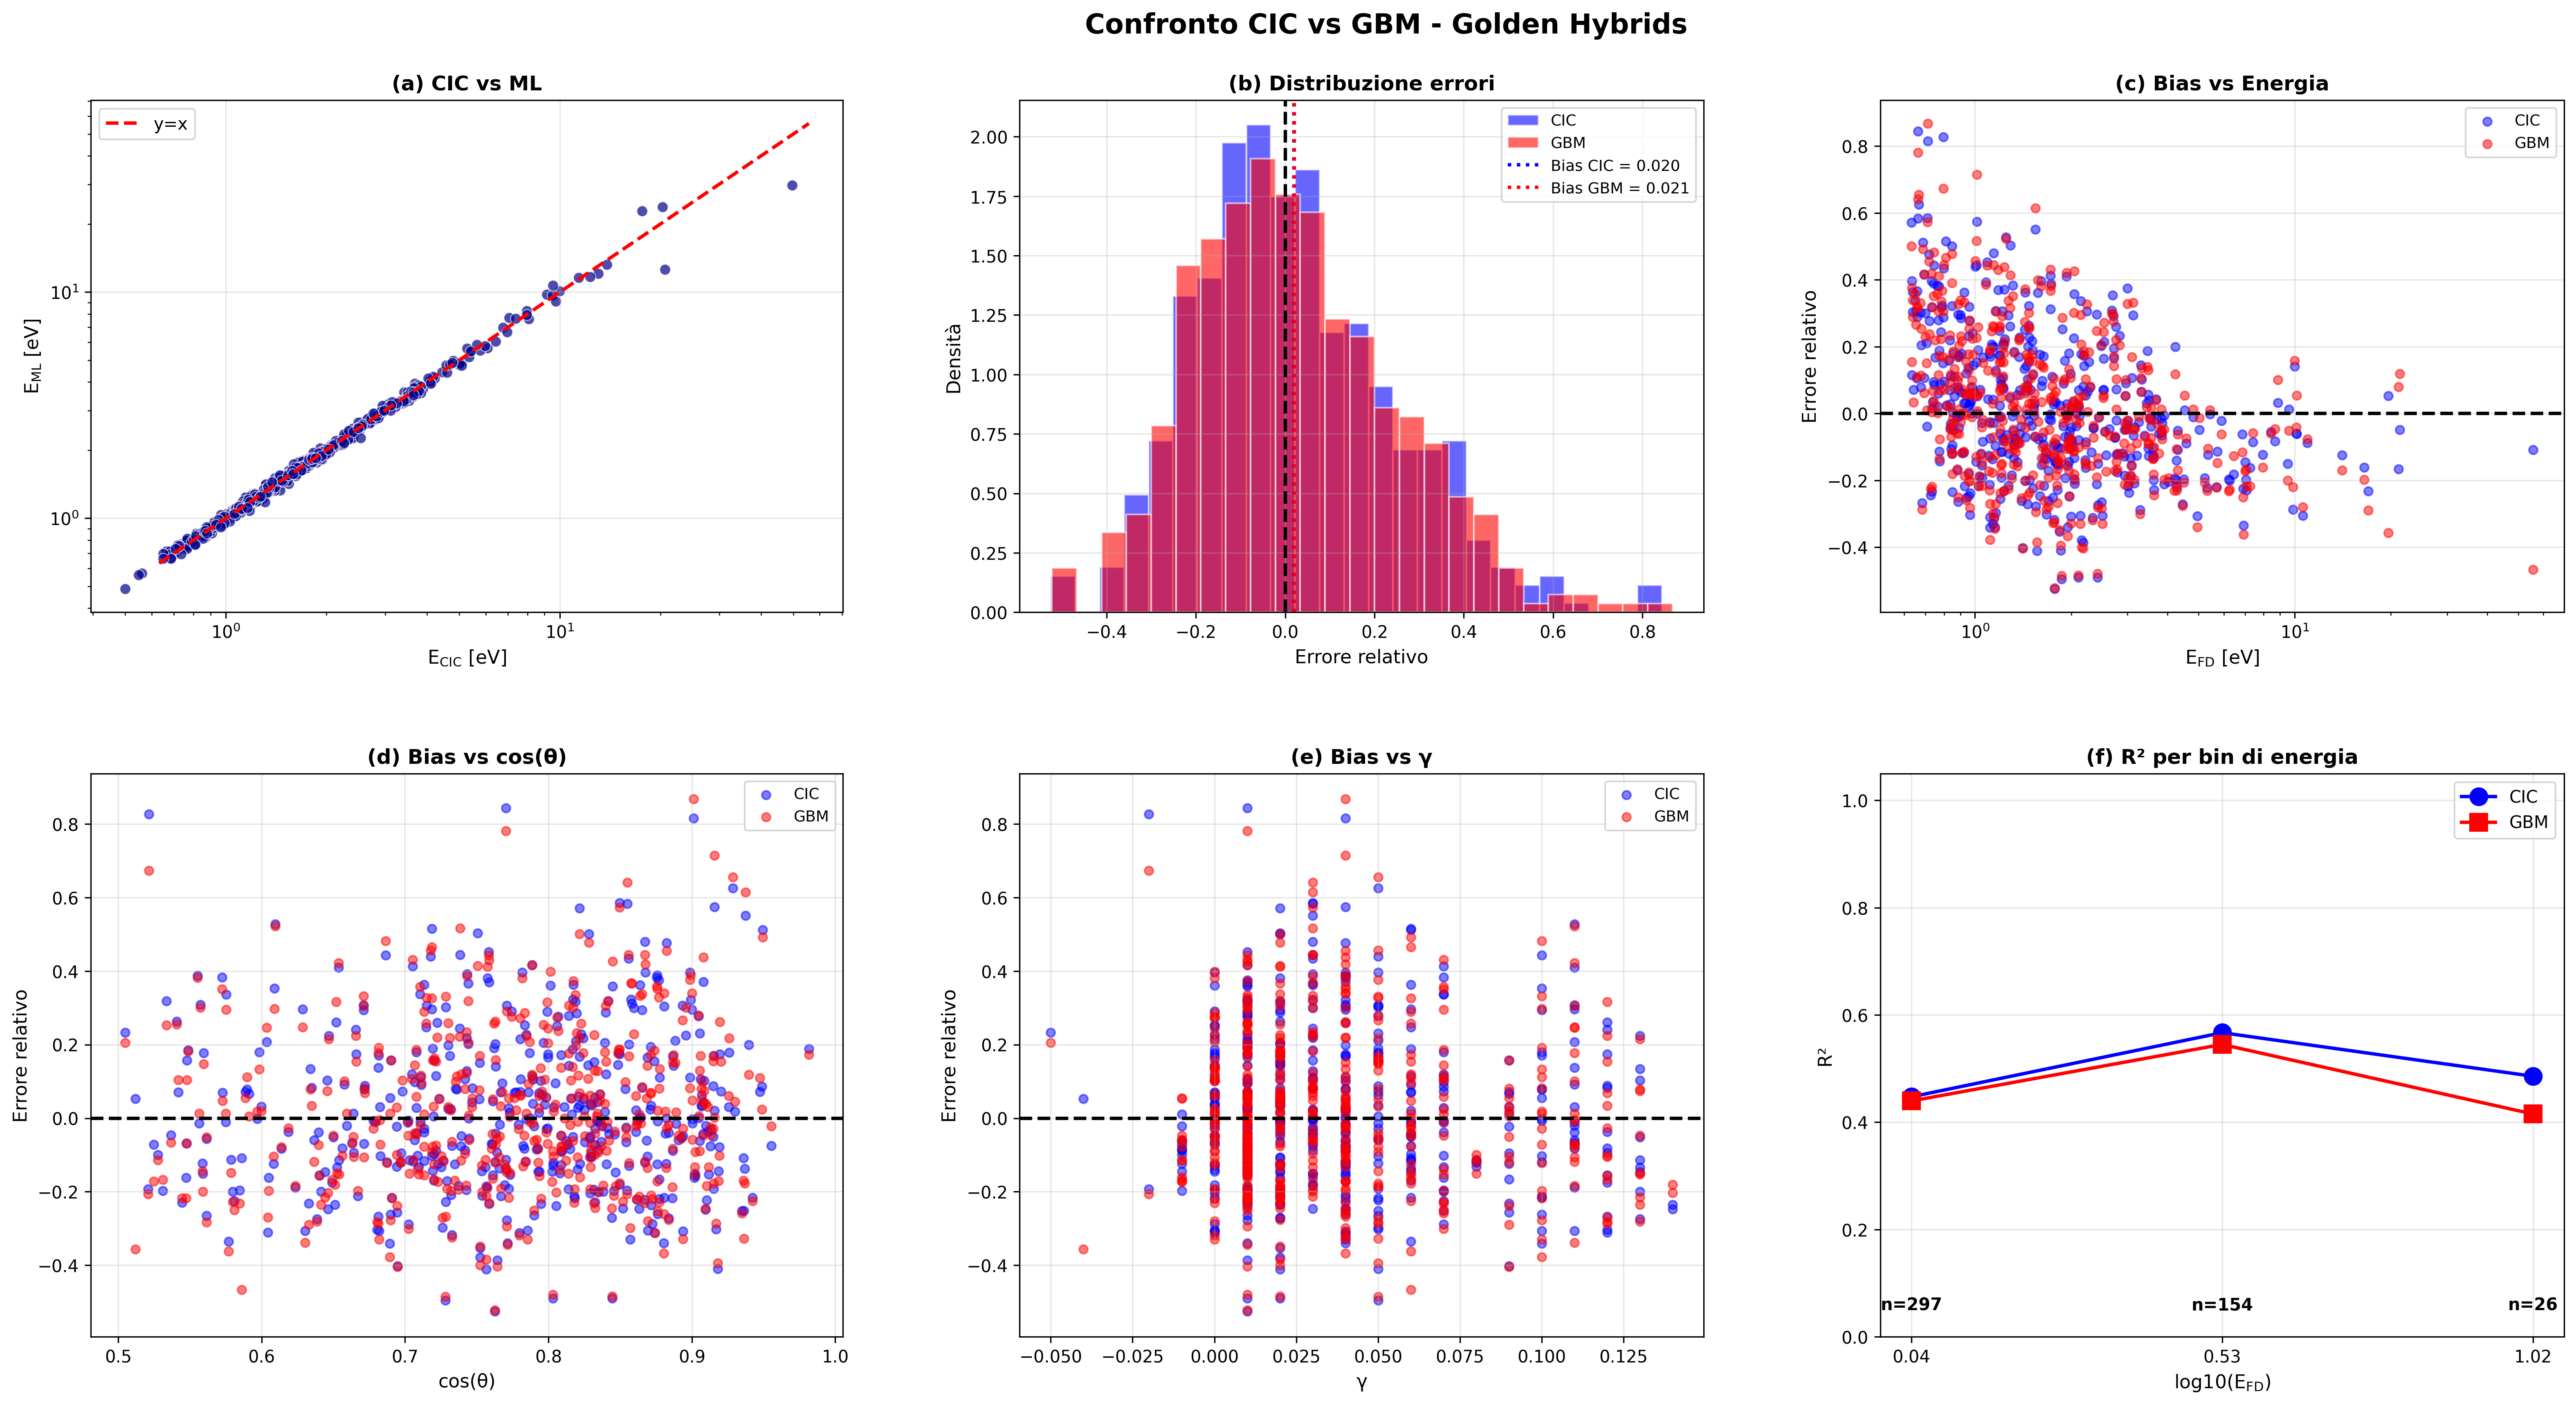
\includegraphics[width=\textwidth]{confronto_CIC_vs_ML_golden.png}
\caption{Confronto finale}
\label{default}
\end{center}
\end{figure}

\end{frame}

\begin{frame}{Sviluppi futuri e Miglioramenti}
Per migliorare i risultati ottenuti in questa analisi, si potrebbe pensare ad una ricerca a griglia dei migliori parametri associati ai metodi ML. Questo perché ogni modello è governato da iper-parametri diversi, un'operazione di ottimizzazione (\emph{cross-validation}) degli stessi porterebbe a modelli sempre più precisi.
\bigskip

Un altro modo per andare oltre quanto fatto in questo progetto sarebbe quello di costruire delle reti neurali che lavorano direttamente sui dati "grezzi" del rivelatore di superficie (ad esempio le tracce temporali dei segnali nelle singole stazioni, organizzate in griglie spaziali), al fine di ridurre la dipendenza dalla ricostruzione standard e dalla conseguente propagazione degli errori. Questo approccio permetterebbe di bypassare completamente la ricostruzione della LDF (e quindi le variabili derivate come $\beta$ e $\gamma$), consentendo al modello di apprendere autonomamente la morfologia dello sciame. 
\end{frame}

\begin{frame}{Fine}
	\centering
	\Huge Grazie per l'attenzione!
\end{frame}

\end{document}